%%%% Proceedings format for most of ACM conferences (with the exceptions listed below) and all ICPS volumes.
\documentclass[sigconf]{acmart}

\settopmatter{printacmref=false} % Removes citation information below abstract
\renewcommand\footnotetextcopyrightpermission[1]{} % removes footnote with conference information in first column
\pagestyle{plain} % removes running headers

\usepackage{listings,xcolor}
%\usepackage[section]{placeins}

\definecolor{dkgreen}{rgb}{0,.6,0}
\definecolor{dkblue}{rgb}{0,0,.6}
\definecolor{dkyellow}{cmyk}{0,0,.8,.3}

\lstset{
  language        = php,
  basicstyle      = \small\ttfamily,
  keywordstyle    = \color{dkblue},
  stringstyle     = \color{red},
  identifierstyle = \color{dkgreen},
  commentstyle    = \color{gray},
  emph            =[1]{php},
  emphstyle       =[1]\color{black},
  emph            =[2]{if,and,or,else},
  emphstyle       =[2]\color{dkyellow}}
\usepackage{booktabs}


% Copyright
\setcopyright{none}

\begin{document}
\title{SOEN7481 Fall 2018: Project Report}
\subtitle{Replicating the paper "How not to structure your database-backed web applications: a study of performance bugs in the wild" by Junwen Yang et al.}

\author{Yann Kerichard}
\affiliation{%
  \institution{Concordia University}
  \city{Montreal}
  \state{Quebec}
  \country{Canada}
}

\author{Yousef Saatchi}
\affiliation{%
  \institution{Concordia University}
  \city{Montreal}
  \state{Quebec}
  \country{Canada}
}

\author{Gagandeep Kaur}
\affiliation{%
  \institution{Concordia University}
  \city{Montreal}
  \state{Quebec}
  \country{Canada}
}

\author{Gagandeep Singh}
\affiliation{%
  \institution{Concordia University}
  \city{Montreal}
  \state{Quebec}
  \country{Canada}
}

\author{Karanvir Singh Sidhu}
\affiliation{%
  \institution{Concordia University}
  \city{Montreal}
  \state{Quebec}
  \country{Canada}
}

\author{Adrien Poupa}
\affiliation{%
  \institution{Concordia University}
  \city{Montreal}
  \state{Quebec}
  \country{Canada}
}


\begin{abstract}
These days most of the web applications are using ORM framework for persistent data storage in databases. ORM framework hides how the queries are fired and executed, so making things a little complicated. In this paper the authors tried to find solutions to the various issues faced during working with the projects using large persistent data and build upon ORM framework. The authors considered 12 representative ORM applications, 9 ORM performance anti-patterns found by studying the bugs listed for them and with the help of profiling the updated versions of the applications. The authors also manually fix 64 performance issues and obtained speed ups by changing only few lines of code. It is also mentioned that the authors achieved 2 to 39 times speed up, by just changing a few lines of code. Thus, in order to replicate the paper, we have evaluated three projects based on the Laravel \cite{laravel} framework: Monica \cite{monica}, Cachet \cite{cachet} and Attendize \cite{attendize}. We have profiled these projects with the help of the DebugBar package \cite{debugbar} and the Telescope package \cite{telescope}. We went through their bug tracking system to get an idea about how they are working, performing  and can be scaled. We have followed the steps taken by the authors. We fixed performances issues and API misuses by removing duplicate queries, solving the N+1 problem, fixing the lack of pagination and database issues to achieve speed-ups and performance improvements, measured the efficiency of the fixes with jMeter and sent pull requests to the applications' repositories.

\end{abstract}

\keywords{Performance anti-patterns, Object-Relational Mapping, Database-backed Applications, Bug study, Laravel, PHP, MySQL, Eloquent, DebugBar, Telescope, Monica, Cachet, Attendize, jMeter}

\maketitle

\section{Introduction}
ORM frameworks are gaining popularity and have implementations in mostly all common general-purpose languages. But they also have some concerns about the performance and scalability. One of the concerns is that since ORM frameworks hide the query generation and execution details, it becomes difficult to optimize the interaction between the applications and the underlying database. Even executing queries efficiently is a concern. And the main worry is regarding testing since in-house testing is usually done with a small amount of data compared to the data the projects usually encounter when they are actually deployed. Moreover, the performance problems faced on the client side have been studied well but the server side concerns were not. In this project we will be using the methodology of the authors of the original paper. The authors targeted three main questions about ORM applications:
\begin{enumerate}
\item How well the real world back-end applications perform when the amount of data increases?
\item What are the common root causes of performance and scalability issues in such applications?
\item What could be the potential solutions of such problems?
\end{enumerate}
Thus, we will be taking into account these questions. The authors did two-pronged empirical study on the 12 Rails applications that can be categorized into 6 categories. They examined 140 fixed performance issues with the help of bug-tracking systems of these 12 applications. They also performed profiling and code review of these applications. They found solutions and fixes for the research questions to gain performance and speed ups. In this report, we replicate the same study for three Laravel applications: Monica, Cachet and Attendize. We improve the performance of these applications, measure the results and identify bug patterns such as duplicate queries, the N+1 problem, the lack of pagination and database issues.

\section{Motivations}
Studies have shown that nearly half of the users expect a website to load in less than 2 seconds and will abandon a website if it is not loaded within 3 seconds \cite{siteleave}. A big part of the time spent by a server to load a web page depends on the time used to extract data from the database. Nowadays, more and more developers in the industry use ORM frameworks to not having to deal with the SQL queries. Moreover, there are very few papers studying this subject, therefore our study presents a real interest. In our paper we decided to focus on a widely used technology in the world today: PHP. By studying performance issues with a PHP ORM framework, we potentially hit 79.0\% of all the websites whose server-side programming language we know \cite{w3tech}. Furthermore, in addition to being designed to allow developers to learn about the differences in performance between ORM frameworks and SQL queries, our paper also wants to provide them solutions in order to fix the performance issues.

\begin{figure*}[ht!]
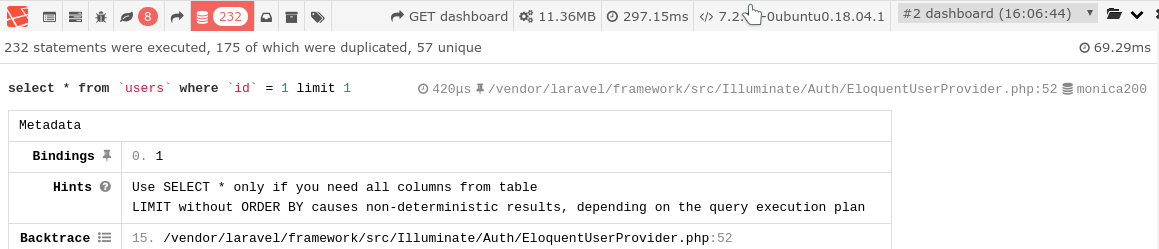
\includegraphics[width=\textwidth]{debugbar2}
\caption{Screenshot of the DebugBar}
\label{debugbar}
\end{figure*}
\begin{table*}[ht!]
\begin{tabular}{|l|l|l|l|l|l|}
\hline
\textbf{Project} & \textbf{Stars} & \textbf{Contributors} & \textbf{Commits} & \textbf{Issues} & \textbf{Pull Requests} \\ \hline
Monica           & 6,247                    & 140                             & 1,205                      & 334                       & 21                               \\ \hline
Cachet           & 8,976                    & 152                             & 6,430                      & 139                       & 41                               \\ \hline
Attendize        & 2,231                    & 49                              & 810                        & 107                       & 9                                \\ \hline
\end{tabular}
\caption{Statistics for the three projects as of December, 7\textsuperscript{th} 2018}
\label{statistics}
\end{table*}

\section{Techniques Used}
We have selected three popular open sources projects that use the Laravel framework and its ORM Eloquent. Our criteria for selection were:
\begin{enumerate}
\item Popularity: the software had to have a large the number of stars in GitHub.
\item Maintenance: the software had to be actively maintained.
\item Maturity: the software had to be over a year old.
\item Eloquent: the software had to use Eloquent so that we could identify eventual ORM misuses.
\end{enumerate}
\noindent Based on those criteria, we have selected the following packages:
\begin{enumerate}
\item Monica: an open source personal CRM, that remembers everything about one's friends and family. It helps one to organize the social interactions with their loved ones \cite{monica}
\item Cachet: an open source status page system. It is used by companies all over the world to communicate downtime and system outages to their customers, teams and shareholders \cite{cachet}
\item Attendize: an open-source ticket selling and event management platform. It has a wide array of features aimed at making organizing events as effortless as possible \cite{attendize}.
\end{enumerate}
\noindent Table \ref{statistics} shows the statistics for each project as of December, 7\textsuperscript{th} 2018. We seeded the databases with 200 records, 2,000 records and 20,000 records like in the original paper to see the impact in terms of performance of a growing database. To do so, we used database seeders. The DebugBar \cite{debugbar} is used. This is a package for Laravel \cite{laravel}, available on Composer \cite{debugbarpackage}, the PHP package manager. A screenshot of the DebugBar is shown in figure \ref{debugbar}. We will evaluate the queries shown in the Queries tab of the bar to see the queries run on each page of the application. It is capable of detecting seven performance bug patterns for the queries:
\begin{enumerate}
\item Use SELECT * only if you need all columns from table.
\item ORDER BY RAND() is slow, try to avoid if you can.
\item The != operator is not standard. Use the <> operator to test for inequality instead.
\item The SELECT statement has no WHERE clause and could examine many more rows than intended.
\item LIMIT without ORDER BY causes non-deterministic results, depending on the query execution plan.
\item An argument has a leading wildcard character: ... The predicate with this argument is not sargable and cannot use an index if one exists.
\item Duplicated statements (e.g. 9 statements were executed, 2 of which were duplicated, 7 unique).
\end{enumerate}
\noindent We also used the Telescope package \cite{telescope} to achieve the same purpose. A screenshot of the Telescope package is shown in Figure \ref{telescope}. The two packages complete each other; the DebugBar is attached to every page allowing the developer to see the relevant information once for every page whereas Telescope lives in its own folder but logs all the queries and requests for later. Finally, we used jMeter \cite{jmeter} to measure the loading time of the pages before and after a fix.

\begin{figure*}[ht!]
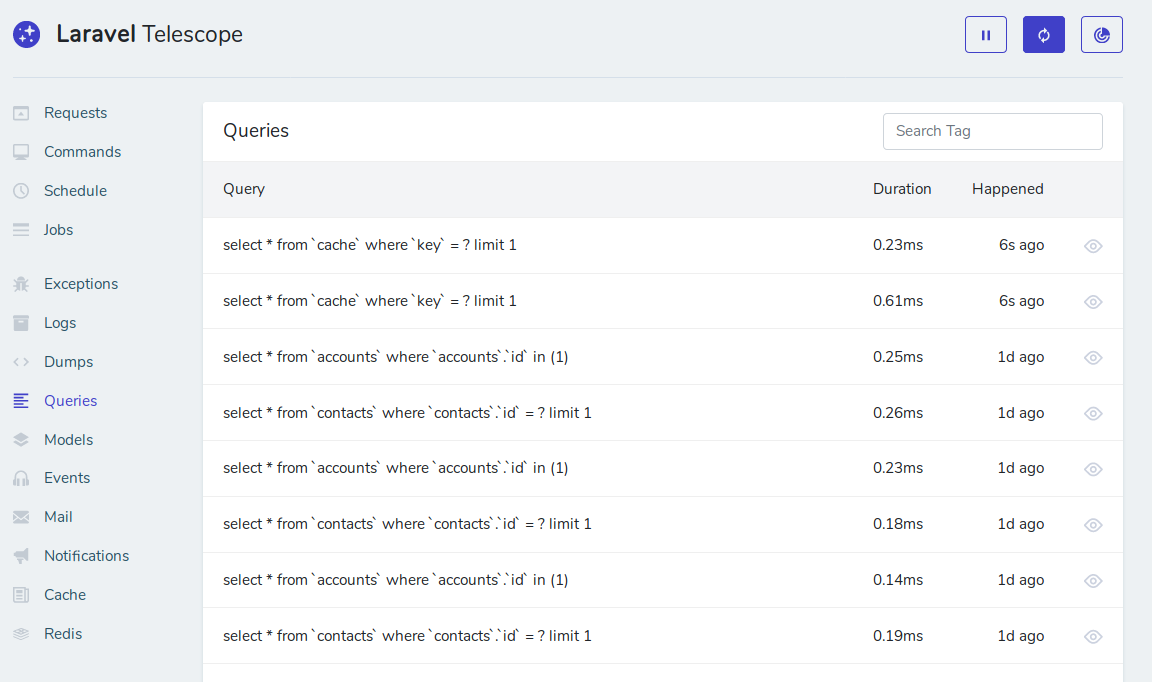
\includegraphics[width=0.6\textwidth]{telescope}
\caption{Screenshot of Laravel Telescope}
\label{telescope}
\end{figure*}

\section{Seeding the Database}
Database seeding is the process done initially that consists of seeding of a database with data \cite{seeding}. When seeding a database, an initial set of data is provided to a database during or after the installation of a software. Dummy data is used to fill the database with fake but valid data. This is useful to evaluate the behavior of an application like in real life, where the number of entries in the database will grow over time. Laravel explicitly supports database seeding \cite{laravelseeding}. Thus, instead of using "real world data" in a way that is not described in the original paper, we chose to use seeders for our three applications. The availability of those seeders was variable depending on the application.
\subsection{Monica}
In Monica, there was a seeder available, \texttt{FakeContentTableSeeder}. While it was useful, we soon discovered that it would only run with an empty database, that is, right after the installation of the software. By default, it would create a random number of contacts between 60 and 100. This is not enough as we wanted to generate 200, 2,000 and 20,000 contacts. Also, the generation of those mock contacts relied on the RandomUser website \cite{randomuser}, whose API is limited to returning 5,000 fake people at once \cite{randomuserdoc}. Therefore, we needed to run the seeder four times, generating 5,000 contacts each time. We fixed the seeder and sent a pull request to the Monica repository \cite{prseedmonica}, that has been merged in the main repository . The seeder could not be run more than once because it was first creating a new account, adding the contacts, then creating a second account. When relaunching the seeder, it would randomly get a model instance, that could belong to account number 2 whereas the seeder was run as account number 1. Thus, the seeder was trying to access a resource with the wrong user identifier.
\subsection{Cachet}
For Cachet, the seeder available \cite{cachetseeder} was not capable of generating the required number of  data objects that we needed for this project (200, 2,000 and 20,000)  and various tables in the database had primary key constraints associated with them. Inserting random data or dummy data into the database was violating these constraints. Therefore, to insert the required data into the database of Cachet, we went through the code of the seeder to make the necessary changes. While reviewing the code of the demo seeder provided, we found out that if we alter the given loop statements and make them iterate for the required number of times (200, 2,000 and 20,000), we could generate the data as per our requirements. And to handle the problem of primary key constraint  violation, we associated the loop variable with the unique fields in the database. 
\begin{figure}
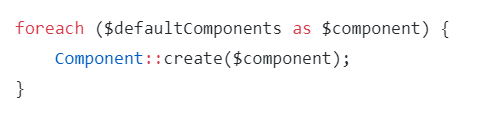
\includegraphics[]{Previous_Code}
\caption{Screenshot of the Cachet seeders old code}
\label{Previous_Code}
\end{figure}
\begin{figure}
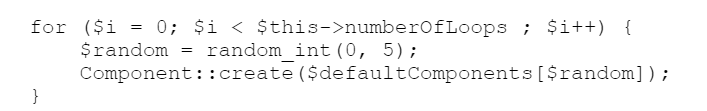
\includegraphics[width=0.5\textwidth]{Updated_Code}
\caption{Screenshot of the Cachet seeders updated code}
\label{Updated_Code}
\end{figure}

\subsection{Attendize}
For the Attendize project, after analyzing the database and different routes of the application using Laravel DebugBar, we identified the most frequently used database tables in the selected pages. The analyzed routes are as follows.
\begin{itemize}
\item \texttt{/organiser/1/dashboard}
\item \texttt{/organiser/1/events}
\item \texttt{/event/2/dashboard}
\item \texttt{/event/2/tickets}
\item \texttt{/event/2/attendees}
\end{itemize}
Based on our analysis, two of the most frequently queried tables are \texttt{organizers} and \texttt{events}, which considering the purpose of the application as an event organizer, is not surprising. Below is a list of the most tables we selected to seed based on the frequency of their usage in the application.
\begin{itemize}
\item \texttt{users}
\item \texttt{organizers}
\item \texttt{events}
\item \texttt{accounts}
\item \texttt{tickets}
\item \texttt{orders}
\item \texttt{orderItems}
\item \texttt{attendees}
\end{itemize}
Since there were no seeders available for the purpose of our tests in the project, we had to prepare them from scratch. We preserved the same pattern we used for other applications for the seeders of this application and populated the database in three phases, first with 200 records in each table, then 2,000 records and finally 20,000 records.

\subsection{Populating the Database}
After seeding the database for each of the three projects, we noticed a difference while comparing the size of the databases, as shown in figure \ref{dbrecords}. Monica has the highest size by far, mostly because the project was not made to scale with a 20,000 contacts database, according to one of the main contributors \cite{MonicaPagination}. Therefore, Monica's database is not aimed to be scalable, and that is why we found that there is room for improvement. Moreover, Monica's database contains a lot of information related to each contact, such as events, gifts purchase, etc... On the other side, Attendize and Cachet contain less data due to the fact that each entry in the database is less customizable. Overall, we noticed that for the three projects, the size of the database increases almost linearly with the number of records. Once the database was filled, we analyzed the performance of each project.

\begin{figure}[t!]
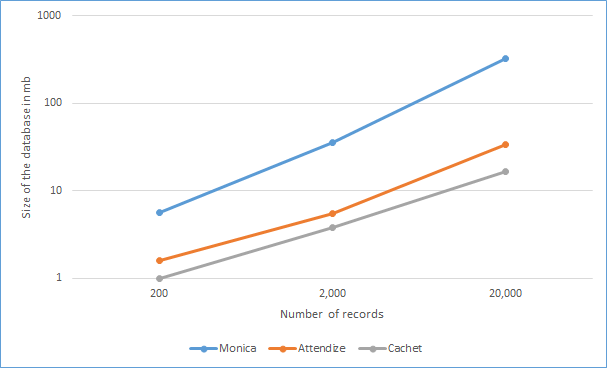
\includegraphics[width=0.4\textwidth]{dbrecords}
\caption{Size of the database for each project}
\label{dbrecords}
\end{figure}

\section{Performance Review}
The performance review will be detailed into 3 parts. The first part is aimed to provide you some insights about the possible analysis tools, and the one we chose: jMeter. Secondly, we will explain the methodology we used to find performance issues, with tickets analysis, for each project. Finally, the third part will be dedicated to performance analysis for each project, both in terms of time and number of requests.

\subsection{Analysis Tools}
To measure the performance of our project, we used the application jMeter. It is an Apache project open source software that can be used to measure the performance and test the functional behavior of variety of services, but the main focus is on the web applications. It can be used for testing static and dynamic resources, measuring and testing the performance of different types of applications, servers, and so on. It can also be used for functional testing as well. The architecture of jMeter is based on plugins. There are 64 plugins available for jMeter. It is not a browser but looks like it and does not support all the actions that can be performed a normal browsers. Extensive documentation is available for the installation and use of jMeter. It is also used for the analysis of the performance of web applications or variety of other services. This means testing the web application against heavy load (in our case large databases). There are various advantages of using jMeter like it is open source, it has a user friendly GUI, it is platform independent, there is a provision of visualizing the test results, its installation is easy, it is highly extensible, has good testing capabilities and it offers support for multi-protocols. In our project, we also had the possibility to use the Laravel DebugBar and Laravel Telescope to measure performances. However, jMeter has the advantage that it is completely independent from the project that is running, so it has absolutely no impact on application's performance. In contrary, Laravel DebugBar and Laravel Telescope are still Laravel components, so they still add some additional time costs when running projects, even though those could be negligible.

\subsection{Tickets Selection}
In order to determine the performance issues related to each project, we reproduced the method used in the paper \cite{paper}. So, we went through each application's bug-tracking system and we looked for tickets containing the keywords performance, slow, or optimization. Then, by analyzing those tickets an by running the application, we could identify the major problems for each project.\\

\subsubsection{Monica}~\\
Concerning Monica, we obtained a list of 7 tickets. Among them, two tickets are unresolved and one is irrelevant. However, we could identify the heaviest web pages in term of loading time. Those tickets were reporting performance issues related to database overload, mostly concerning 2 pages. The first page was displaying the contact list, and, we noticed that the problem was coming from the fast that the page had not pagination. It was loading all the contacts of the database related to a specific user. So in the case where this user had 1,000 contacts, the 1,000 contacts were loaded on one single page.\\
\begin{table*}[t!]
\begin{tabular}{|l|l|l|}
\hline
\multicolumn{1}{|c|}{\textbf{Keyword}} & \multicolumn{1}{c|}{\textbf{Bug link}}         & \multicolumn{1}{c|}{\textbf{Title}}                                     \\ \hline
performance                            & \url{https://github.com/monicahq/monica/pull/227}    & Refactoring PeopleController for better performance and readability     \\ \hline
performance                            & \url{https://github.com/monicahq/monica/pull/388}    & issues/345 - /people slow with many contacts                            \\ \hline
slow                                   & \url{https://github.com/monicahq/monica/pull/209}    & Fixing some relationship inconsistencies and reducing dashboard queries \\ \hline
slow                                   & \url{https://github.com/monicahq/monica/issues/1992} & Pagination on the people page (/people)                                 \\ \hline
optimization                           & \url{https://github.com/monicahq/monica/pull/1321}   & Optimization for getting list of countries                              \\ \hline
optimization                           & \url{https://github.com/monicahq/monica/issues/204}  & Database Changes and Optimisation                                       \\ \hline
query                                  & \url{https://github.com/monicahq/monica/pull/228}    & Eager Loading People                                                    \\ \hline
\end{tabular}
\caption{Monica tickets}
\label{Monicatickets}
\end{table*}

\subsubsection{Cachet}~\\
For Cachet, we gathered a list of 14 tickets: 4 of them were irrelevant, and only 1 was unresolved. We could then easily determine 4 pages causing performance issues.\\

\begin{table*}[t!]
\begin{tabular}{|l|l|l|}
\hline
\multicolumn{1}{|c|}{\textbf{Keyword}} & \multicolumn{1}{c|}{\textbf{Bug link}}         & \multicolumn{1}{c|}{\textbf{Title}}                                         \\ \hline
performance                            & \url{https://github.com/CachetHQ/Cachet/issues/17}   & Caching                                                                     \\ \hline
performance                            & \url{https://github.com/CachetHQ/Cachet/pull/382}    & Enhance settings performance queries                                        \\ \hline
performance                            & \url{https://github.com/CachetHQ/Cachet/pull/2040}   & Metric repository perf                                                      \\ \hline
performance                            & \url{https://github.com/CachetHQ/Cachet/pull/2220}   & Scheduled maintenance refactor                                              \\ \hline
slow                                   & \url{https://github.com/CachetHQ/Cachet/issues/2566} & Please optimize front end                                                   \\ \hline
slow                                   & \url{https://github.com/CachetHQ/Cachet/issues/2617} & Metric loading takes long time                                              \\ \hline
slow                                   & \url{https://github.com/CachetHQ/Cachet/issues/2001} & cachet front page super slow, stalling                                      \\ \hline
slow                                   & \url{https://github.com/CachetHQ/Cachet/issues/576}  & curl\_multi\_exec - too slow                                                \\ \hline
optimization                           & \url{https://github.com/CachetHQ/Cachet/issues/209}  & Don't Missuse The Return Annotation                                         \\ \hline
query                                  & \url{https://github.com/CachetHQ/Cachet/issues/3004} & Should Component/tag be a ManyToMany relation?                              \\ \hline
query                                  & \url{https://github.com/CachetHQ/Cachet/pull/2266}   & Metrics: Calculation set to average always sums                             \\ \hline
query                                  & \url{https://github.com/CachetHQ/Cachet/issues/1900} & Non-optimal app layer iteration in MetricRepository                         \\ \hline
query                                  & \url{https://github.com/CachetHQ/Cachet/pull/1323}   & Call first() on the query itself                                            \\ \hline
query                                  & \url{https://github.com/CachetHQ/Cachet/pull/595}    & Refactored the way incidents are pulled out of the database on the homepage \\ \hline
\end{tabular}
\caption{Cachet tickets}
\label{Cachettickets}
\end{table*}

\subsubsection{Attendize}~\\
Finally, by analyzing Attendize's bug-tracking reporting system, we were only able to find 4 tickets using the keywords, and among them, 2 were unresolved, and 2 were irrelevant. We were able to identify that the main performance issues were coming from 4 web pages.

\begin{table*}[t!]
\begin{tabular}{|l|l|l|}
\hline
\multicolumn{1}{|c|}{\textbf{Keyword}} & \multicolumn{1}{c|}{\textbf{Bug link}}            & \multicolumn{1}{c|}{\textbf{Title}}                 \\ \hline
performance                            & \url{https://github.com/Attendize/Attendize/issues/27}  & Compiling scripts and stylesheets                   \\ \hline
slow                                   & \url{https://github.com/Attendize/Attendize/issues/1}   & Image gallery on attendize.com resizing             \\ \hline
query                                  & \url{https://github.com/Attendize/Attendize/issues/70}  & Unable to fill up database during installation      \\ \hline
query                                  & \url{https://github.com/Attendize/Attendize/issues/407} & Error when inviting users to an event (VAT related) \\ \hline
\end{tabular}
\caption{Attendize tickets}
\label{Attendizetickets}
\end{table*}

\subsection{Performance Analysis}
\subsubsection{Monica}~\\
Using jMeter, we identified two critical pages that were taking a long time to load in Monica. Those pages were the following:
\begin{enumerate}
\item Contacts: a page that displays a list of all the contacts present in the  database. However, the issue is that this page has no pagination whatsoever, so it loads fast with 200 records but gets slower and slower as the number of records grows.
\item Dashboard: homepage of Monica once the user is logged in. It shows the upcoming events for the following three months (eg: birthdays, custom reminders, etc).
\end{enumerate}
\ \\With jMeter, we have run 100 requests on these two pages for the three databases, before and after the fix. Then, we computed the loading time of those 100 requests to have a higher precision. Figure \ref{loadingtimemonica} shows the average loading time for the two pages.
\begin{figure}[b!]
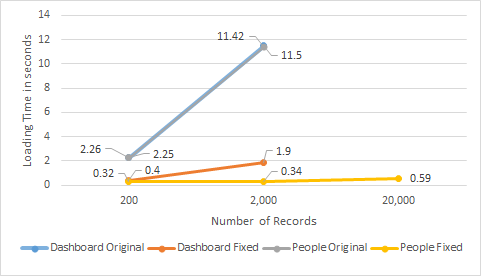
\includegraphics[width=0.5\textwidth]{loadingtimemonica}
\caption{Average loading time in seconds for the two pages as measured by jMeter for Monica}
\label{loadingtimemonica}
\end{figure}
Figure \ref{monicaqueries} shows the number of unique and duplicate queries for those two pages before applying our fixes, that are detailed in section 6. 
\begin{figure}[t!]
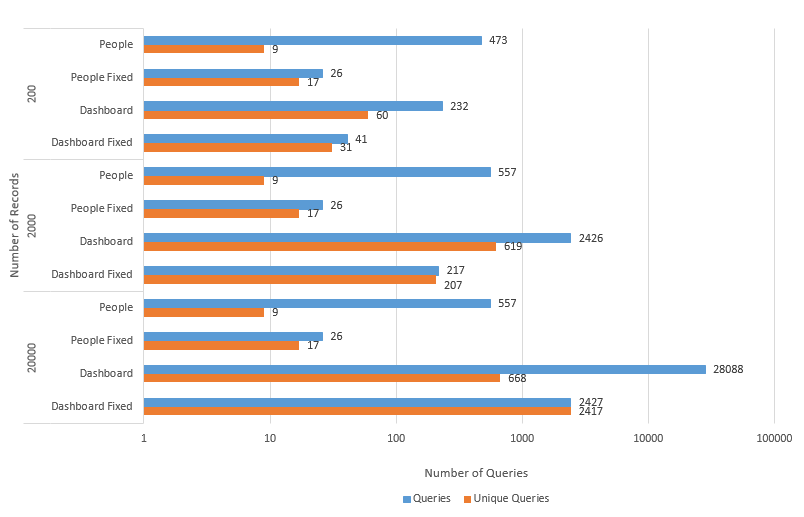
\includegraphics[width=0.5\textwidth]{monicaqueries}
\caption{Number of unique and duplicate queries in Monica depending on the number of records}
\label{monicaqueries}
\end{figure}
Before our fix, we could see a high number of duplicated queries, 98\% of the queries being run more than once in the dashboard page and 75\%  in the people page. As the database grows, the number of queries rises. Our fix reduced this to a constant number of 10 duplicated queries on the dashboard page and 9 duplicated queries on the people page. Those numbers remain constant as the database grows.\newpage
\subsubsection{Cachet}~\\
Using jMeter, we identified four critical pages that were taking a long time to load in Cachet. Those pages were the following:
\begin{enumerate}
\item Index: only page of Cachet that is publicly available. It shows the status of the systems monitored by Cachet and their history. 
\item Dashboard: homepage of Cachet once the user is logged in. It offers an overview of the application to its administrators.
\item Dashboard Components: this page is used to manage the components monitored by Cachet. 
\item Dashboard Incidents: handles the incidents of the components. 
\end{enumerate}
With jMeter, we have run 100 requests on these four pages for the three databases, before and after the fix. Then, we computed the loading time of those 100 requests to have a higher precision. We were not able to measure the loading times for 2,000 and 2,000 records so figure \ref{CachetGraphs} shows the average loading time in seconds for the four pages with the 200 records in the database.
\begin{figure}[b!]
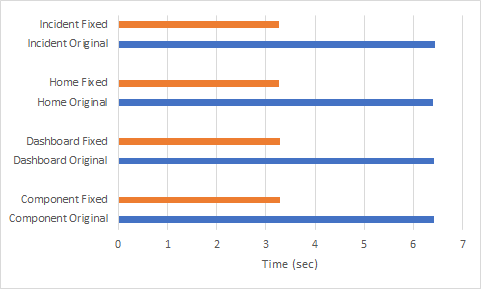
\includegraphics[width=0.3\textwidth]{CachetGraphs}
\caption{Average loading time in seconds for the four pages as measured by jMeter for Cachet}
\label{CachetGraphs}
\end{figure}
Figure \ref{cachetqueries} shows the number of unique and duplicate queries for those four pages before applying our fixes, that are detailed in section 6.
\begin{figure}[t!]
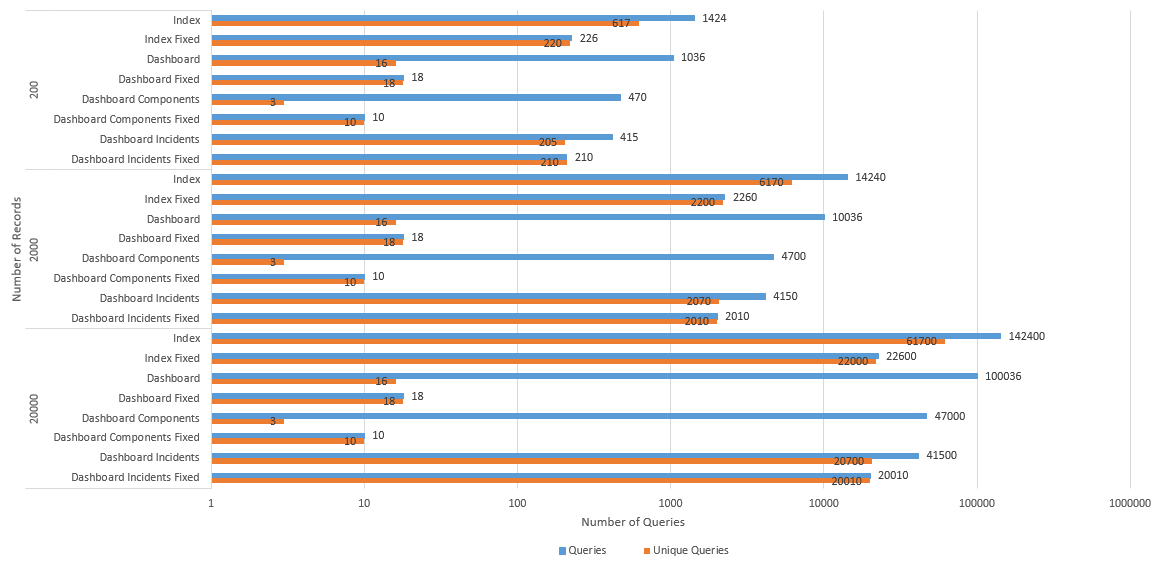
\includegraphics[width=0.5\textwidth]{cachetqueries}
\caption{Number of unique and duplicate queries in Cachet depending on the number of records}
\label{cachetqueries}
\end{figure}
Like in Monica, one can see a high percentage of duplicated queries: 30\% for the index page, 98\% for the dashboard, 99\% for the dashboard components, 50\% for the dashboard incidents. The number of queries increases  as the database grows. Our fixes are the most effective for the dashboard and the dashboard components since the number of queries is now fixed and does not depend on the number of records in the database.
\\
\subsubsection{Attendize}~\\
Using jMeter, we identified four critical pages that were taking a long time to load in Attendize. Those pages were the following:
\begin{enumerate}
\item Dashboard: homepage of Attendize once the user is logged in. It offers an overview of the application to its administrators.
\item Events: lists all the events in the database. 
\item Event Dashboard: the dashboard for a single event. 
\item Event Tickets: shows an overview of the tickets sold and remaining to be sold. 
\end{enumerate}
With jMeter, we have run 100 requests on these two pages for the three databases, before and after the fix. Then, we computed the loading time of those 100 requests to have a higher precision. Figures \ref{attendizeorganiserdashboard}, \ref{attendizeorganiserevent}, \ref{attendizeorganisereventdashboard} and \ref{attendizeorganisereventticket} show the average loading times for the four pages measured with jMeter. One can see that the evolution of the loading times is grows linearly with the growth of the database, and the fixed version loads faster than the original version, albeit slightly. Unlike for the other applications, by default, the number of queries was low and did not increase with the database. Thus, we have been able to remove some duplicated queries but not as much as in Monica or Cachet.
\begin{figure}[b!]
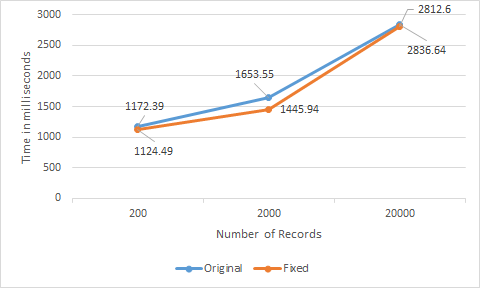
\includegraphics[width=0.5\textwidth]{attendizeorganiserdashboard}
\caption{Average loading time in milliseconds for the Attendize organiser dashboard}
\label{attendizeorganiserdashboard}
\end{figure}
\begin{figure}[b!]
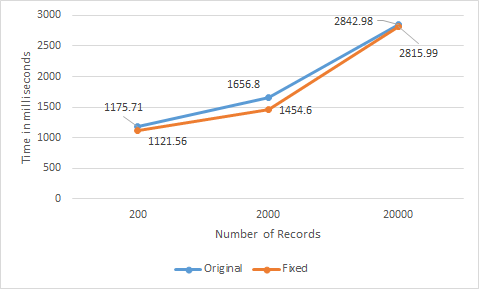
\includegraphics[width=0.5\textwidth]{attendizeorganiserevent}
\caption{Average loading time in milliseconds for the Attendize organiser event}
\label{attendizeorganiserevent}
\end{figure}
\begin{figure}[b!]
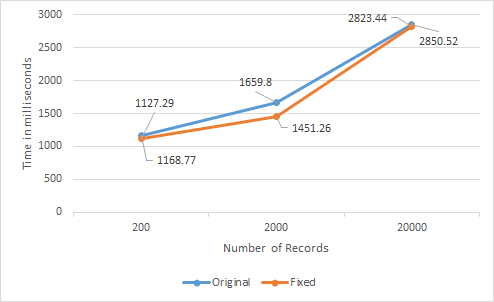
\includegraphics[width=0.5\textwidth]{attendizeorganisereventdashboard}
\caption{Average loading time in milliseconds for the Attendize organiser event dashboard}
\label{attendizeorganisereventdashboard}
\end{figure}
\begin{figure}[b!]
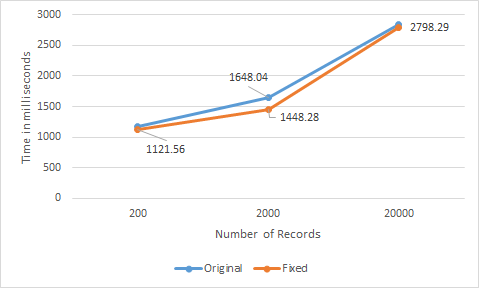
\includegraphics[width=0.5\textwidth]{attendizeorganisereventticket}
\caption{Average loading time in milliseconds for the Attendize organiser event ticket}
\label{attendizeorganisereventticket}
\end{figure}
Figure \ref{attendizequeries} shows the number of unique and duplicate queries for those four pages before applying our fixes, that are detailed in section 6.
\begin{figure}[t!]
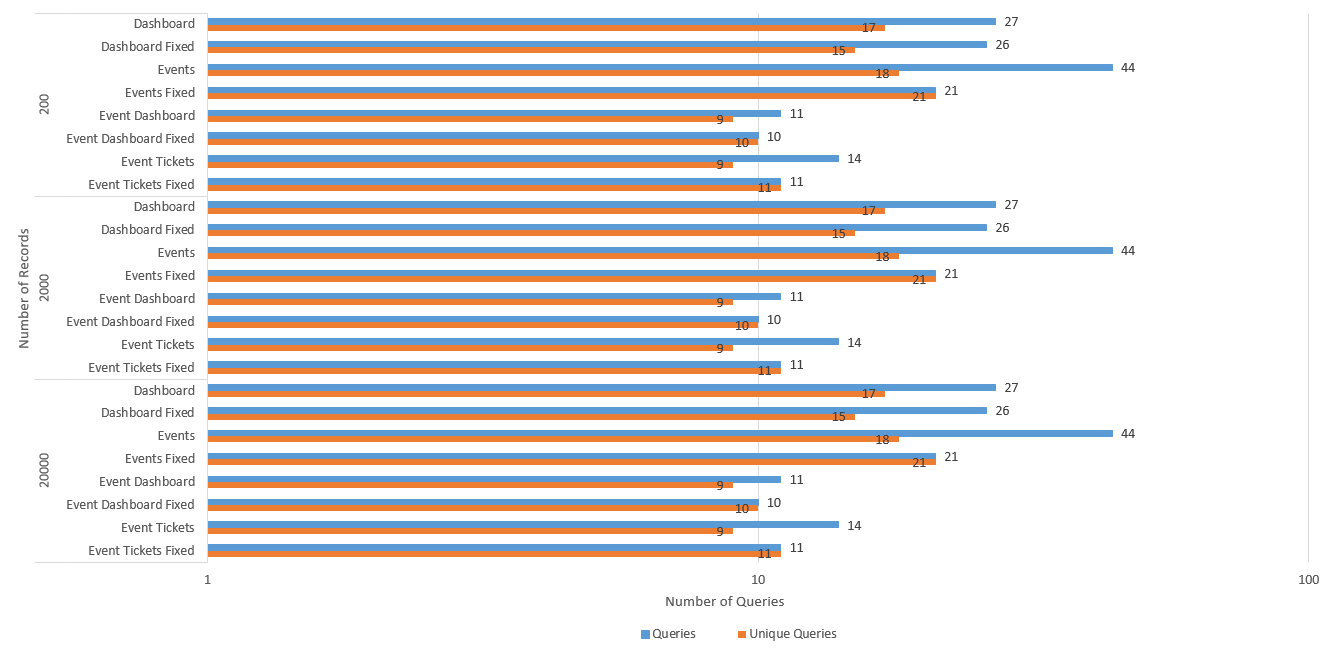
\includegraphics[width=0.5\textwidth]{attendizequeries}
\caption{Number of unique and duplicate queries in Attendize depending on the number of records}
\label{attendizequeries}
\end{figure}
\section{Improving the Performance}
This section details how the performance was improved for the three applications.
\subsection{Monica}
\begin{figure}[t!]
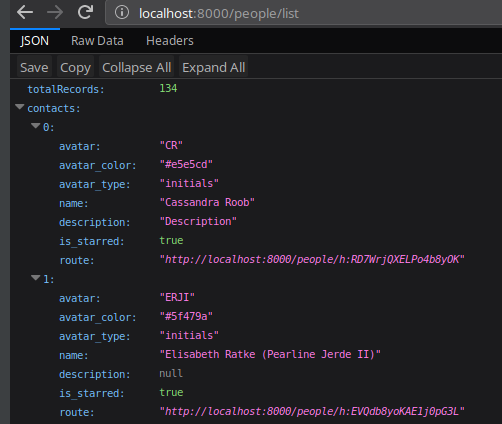
\includegraphics[width=0.4\textwidth]{apimonica}
\caption{New API used by Monica}
\label{apimonica}
\end{figure}
\begin{figure}[t!]
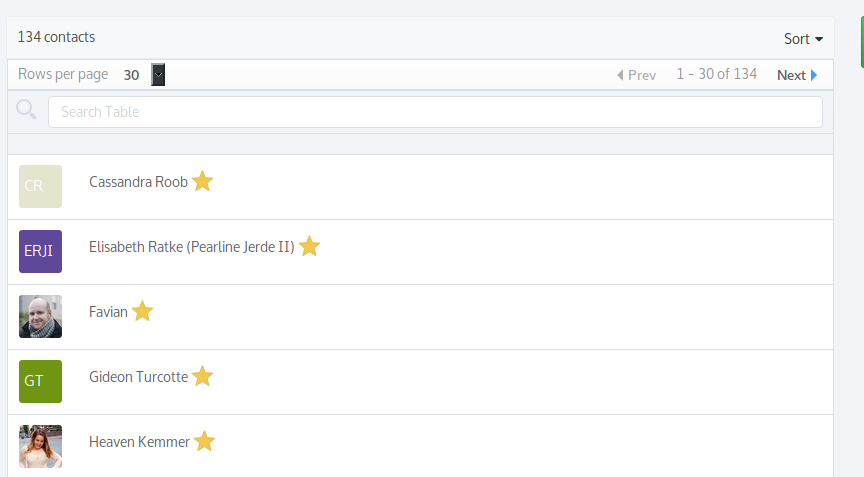
\includegraphics[width=0.5\textwidth]{tablemonica}
\caption{New table for the Monica people page}
\label{tablemonica}
\end{figure}
In Monica, the main issue with the people page was its lack of pagination. This meant that for a small database, say, 200 contacts, the page would load quickly displaying all the contacts at once. On the other hand, with a higher number of contacts, the loading time would increase linearly with the database growth as more and more time is needed to render all the contacts. In this case, the solution is to paginate the results so that the same number of contacts, say, 30, is always displayed regardless of the database size. This way, the loading time of the page remains constant. This problem was already reported in a ticket \cite{MonicaPagination}. We fixed it in a pull request \cite{prpeoplemonica}. We used the vue-good-table component \cite{vgt}: it is a vuejs component that offers a JavaScript data (dynamic) table as shown in figure \ref{tablemonica}. We perform the pagination on the backend so that only 30 results are retrieved for each page through an API as shown in figure \ref{apimonica}. Moreover, the table display is asynchronous, meaning that the user would not be blocked by a long response from the backend. In this pull request, 366 lines have been added, and 118 lines have been removed. For the dashboard, we sent a pull request \cite{prdashboardmonica}. It eager loads the contacts from the reminders table. It also improves the \texttt{getRelatedReal\-Contact} function and replaces two independent MySQL queries with a query that uses a subquery. It also get rids of four duplicate queries performed for every page of the application by loading the data once and storing it in a variable that is available everywhere in the application. In this pull request, 68 lines have been added, and 38 lines have been removed.
\begin{figure}[t!]
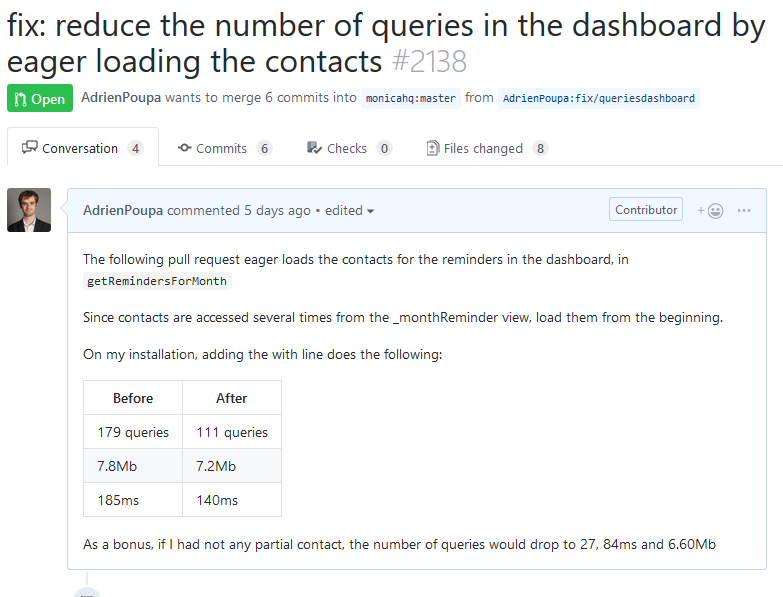
\includegraphics[width=0.4\textwidth]{prdashboard}
\caption{Pull request to remove duplicate queries in the dashboard of Monica}
\label{prdashboard}
\end{figure}
\begin{figure}[t!]
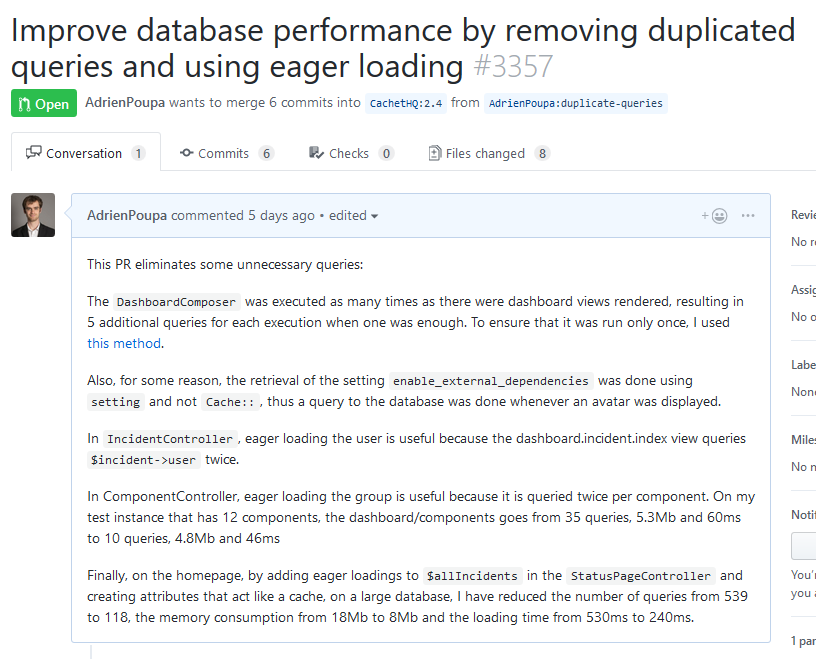
\includegraphics[width=0.5\textwidth]{prcachet}
\caption{Pull request to remove duplicate queries of Cachet}
\label{prcachet}
\end{figure}
\subsection{Cachet}
For Cachet, we removed duplicate queries from the \texttt{Dashboard\-Composer}. In Laravel, a Composer is a component used to share variables among views \cite{viewcomposer}. The \texttt{DashboardComposer} was executed as many times as there were dashboard views rendered, resulting in five additional queries for each execution when one was enough. To ensure that it was run only once, we used a singleton \cite{singleton}. Then, a setting was systematically retrieved from the database instead of using the cache system. Finally, the biggest increase in performance was achieved by eager loading: in \texttt{IncidentController}, eager loading the user is useful because the \texttt{dashboard.incident.index} view queries \texttt{\$incident->user} twice; in \texttt{ComponentController}, eager loading the group is useful because it is queried twice per component. In this pull request, 73 lines have been added, and 15 lines have been removed.
\subsection{Attendize}
In Attendize, we opened a pull request \cite{prattendize} that removes a duplicate query present in the \texttt{FirstRunMiddleware} was eliminated by assigning the value of the query in a variable that is reused. Middlewares are classes executed for each request \cite{middleware}, thus this modification removes an unnecessary query everywhere in the application. In the events tickets page, a query runs 2 or 3 times per event because the function \texttt{getQuantityReservedAttribute} is called several times and calls the database each time the attribute is requested. We have created an attribute directly in the \texttt{Ticket} model, that is set to its value by querying the database once and that is served directly after that. Finally, for the organizer event page, we eager loaded the \texttt{Organiser} and \texttt{Currency} models from the \texttt{Event} model so that every subsequent access to these related models do not trigger a query to the database. In this pull request, 17 lines have been added, and 9 lines have been removed.
\begin{figure}[t!]
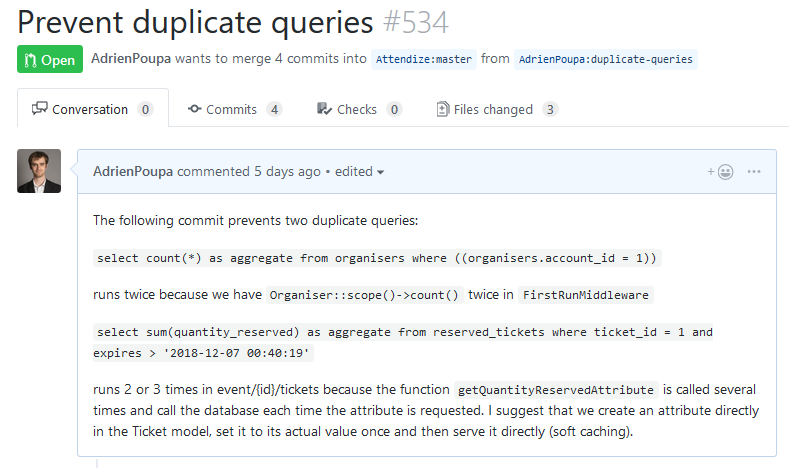
\includegraphics[width=0.5\textwidth]{prattendize}
\caption{Pull request to remove duplicate queries of Attendize}
\label{prattendize}
\end{figure}

\section{Performance Bug Patterns Identified and Their Remedies}
\subsection{Lack of Pagination}
Like in the original paper \cite{paper}, we found that a major source of performance issues was due to the lack of pagination. The people page of Monica is a good example of this: it is not scalable as is since displaying more than a few hundreds of rows is demanding both in terms of MySQL queries and web browser resources. Paginating results is a simple remedy yet a highly efficient one since the number of results to display does not matter; the loading time remains the same. This is even less understandable because Laravel offers support for pagination out of the box \cite{pagination}. It is as simple as adding \texttt{->paginate(15)} to the current query, where \texttt{15} is the number of results we want for a page. Fixes for this include using Laravel's pagination feature or using asynchronous components to display the results (infinite scrolling for example).

\subsection{Duplicate Queries}
Another source for bad performance is duplicate queries. With an ORM such as Eloquent (but the same could be said for Doctrine or Propel), it is easy to get results from the database in a few characters: \texttt{SomeModel::find(1)} where 1 is the identifier of the model you want to retrieve. Thus, coping and pasting several identical model retrievals may not seem to be a bad habit. But in the context of modern web application where databases grow fast, it can quickly become an issue. To fix duplicate queries, one can use either the Laravel DebugBar or Laravel Telescope that log the queries. The DebugBar allows the developer to see the duplicated queries and their stack trace so that it is easier to track the issue. Once the problematic query is found, fixes include:
\begin{enumerate}
\item Assigning the result of the query to a variable and accessing this variable afterwards, instead of performing the same query several times, as seen in figure \ref{variablefix}, that is an excerpt of our fixes for Attendize.
\begin{figure}[h!]
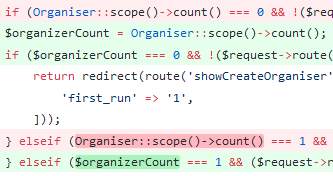
\includegraphics[width=0.3\textwidth]{variablefix}
\caption{Assigning the result of the query to a variable}
\label{variablefix}
\end{figure}
\newpage
Other solutions include putting the results in the attributes of a class and initializing it to given null value so that we know when the value should be initialized from the database. After the initialization, it can be served directly without hitting the database.
\item Eager loading the related models is useful when one knows that for each model found in the database, one of its related models will be accessed systematically. Indeed, Laravel loads the related model each time it is accessed. This is the N+1 problem. Thus, eager loading allows the model to be retrieved once and for all during the initial request \cite{eagerloading}. Figure \ref{eagerload} shows how to eager load a model with a query to avoid the N+1 problem.
\begin{figure}[h!]
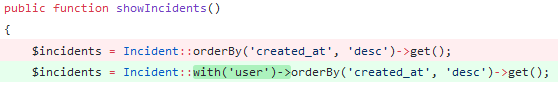
\includegraphics[width=0.5\textwidth]{eagerload}
\caption{Eager loading the \texttt{User} model}
\label{eagerload}
\end{figure}
\end{enumerate}

\subsection{Database Design Issues}
We also found in the three projects under study some performance issues coming from bad database design. As explicitly recognized \cite{monicaticket204} by Monica's main contributor, we found several issues coming back frequently among the three projects. Firstly, database sometimes contain redundant fields, such as field surname in \texttt{contacts} table, which is not needed. Also, another example is the presence of boolean value indicating if another value, already stored is greater than 0, such as the number of kids and \texttt{hasKids} in Monica database. Another bug pattern related to database design could be the naming convention. Column naming is strange in some places. As an example in Monica, there is a \texttt{currencies} table and there is also in table \texttt{gifts} a column named \texttt{valueInDollars}. The main contributor is then explaining that it was just useful at the beginning before supporting multiple currencies.

\subsection{ORM API Misuses}
ORM API misuses is probably the most impacting problem while using an ORM framework. We noticed that, most of the time, developers are getting used to some specific queries and do not realize anymore the impact of each API, in term of number of requests and performance. An example that occurs really frequently in all the projects is when developers are calling an API that will extract unneeded data, coming from unneeded fields. We could easily see this problem with Laravel DebugBar hints system: "Use SELECT * only if you need all columns from table". This may come from developers who are not completely aware of the impact of the API, but it can also come from a bad documentation provided by the ORM framework. Another case that often happens is that developers are trying to combine multiple API to create the same service as provided by an other API, then resulting in the extraction of non-optimal code with unnecessary queries, computations and data.

\section{Related Work}
Our study is strongly related and inspired by the paper \cite{paper} that we studied. Therefore, the related works are pretty much the same. Empirical studies showed that performance bugs take longer time to developer to fix than other types of bugs. Also, our study is targeting performance issues in ORM applications that are mostly related to how application logic interacts with underlying database and are very different from those in general purpose applications. Our study is also related to a previous work \cite{paperInefficiencies} from the same authors of the paper that we replicated. While our paper performs a comprehensive study on all types of performance issues reported by developers, this previous work looked into the database performance of ORM applications and discussed how better database optimization and query translation can improve ORM application performance. Moreover, we also found other studies \cite{paperTechniques,paperBugs} focusing on performance issues in other types of softwares. Detecting and fixing ORM performance anti-patterns require a completely different set of
techniques that understand ORM and underlying database queries.

\section{Future Work}
As improvements, our study could go further in the analysis of specific performance problems in ORM applications, such as
locating unneeded column data retrieval, pushing more computation to the database management system, and query batching. As well as studying and analyzing those problems, some general guidelines could be extracted so that developers avoid repeating the same errors. We could think of replicating the study on other Laravel applications, on other PHP frameworks such as Symfony or CakePHP, or move to a new ecosystem altogether (Python, JavaScript for example).

\section{Conclusion}
Database-backed web applications are widely used and often built using ORM frameworks. Our study focuses on extracting, fixing and providing general guidelines from three active open-source projects based on the Laravel framework and making use of Eloquent. We found performance issues in the three applications despite their popularity and maturity. Our fixes were well received by the community ("That is awesome, I love those optimizations" \cite{prdashboardmonica}, "Thanks for your help @AdrienPoupa this is pretty impressive." \cite{prpeoplemonica}). Apart from the pagination fix, the changes in terms of lines of code were small. Thus, we were able to confirm the results found in the original paper \cite{paper}. It appears the problems faced in the Ruby on Rails ecosystem also exist in PHP, at least within the Laravel framework. After all those experimentations, we noticed that even though ORM have a lot of advantages, such as making querying the database, and, overall, coding easier and faster, they bring performance issues by executing inefficient queries or getting unused data. We were able to link duplicated queries to lower performance by measuring the application loading time with jMeter. However, while it is not systematically the fault of the ORM, often the developers do not use it optimally.

\bibliographystyle{ACM-Reference-Format}

\newpage
\bibliography{bibliography}

\end{document}
 